 \section{Method}

\begin{figure}[t]
\centering
    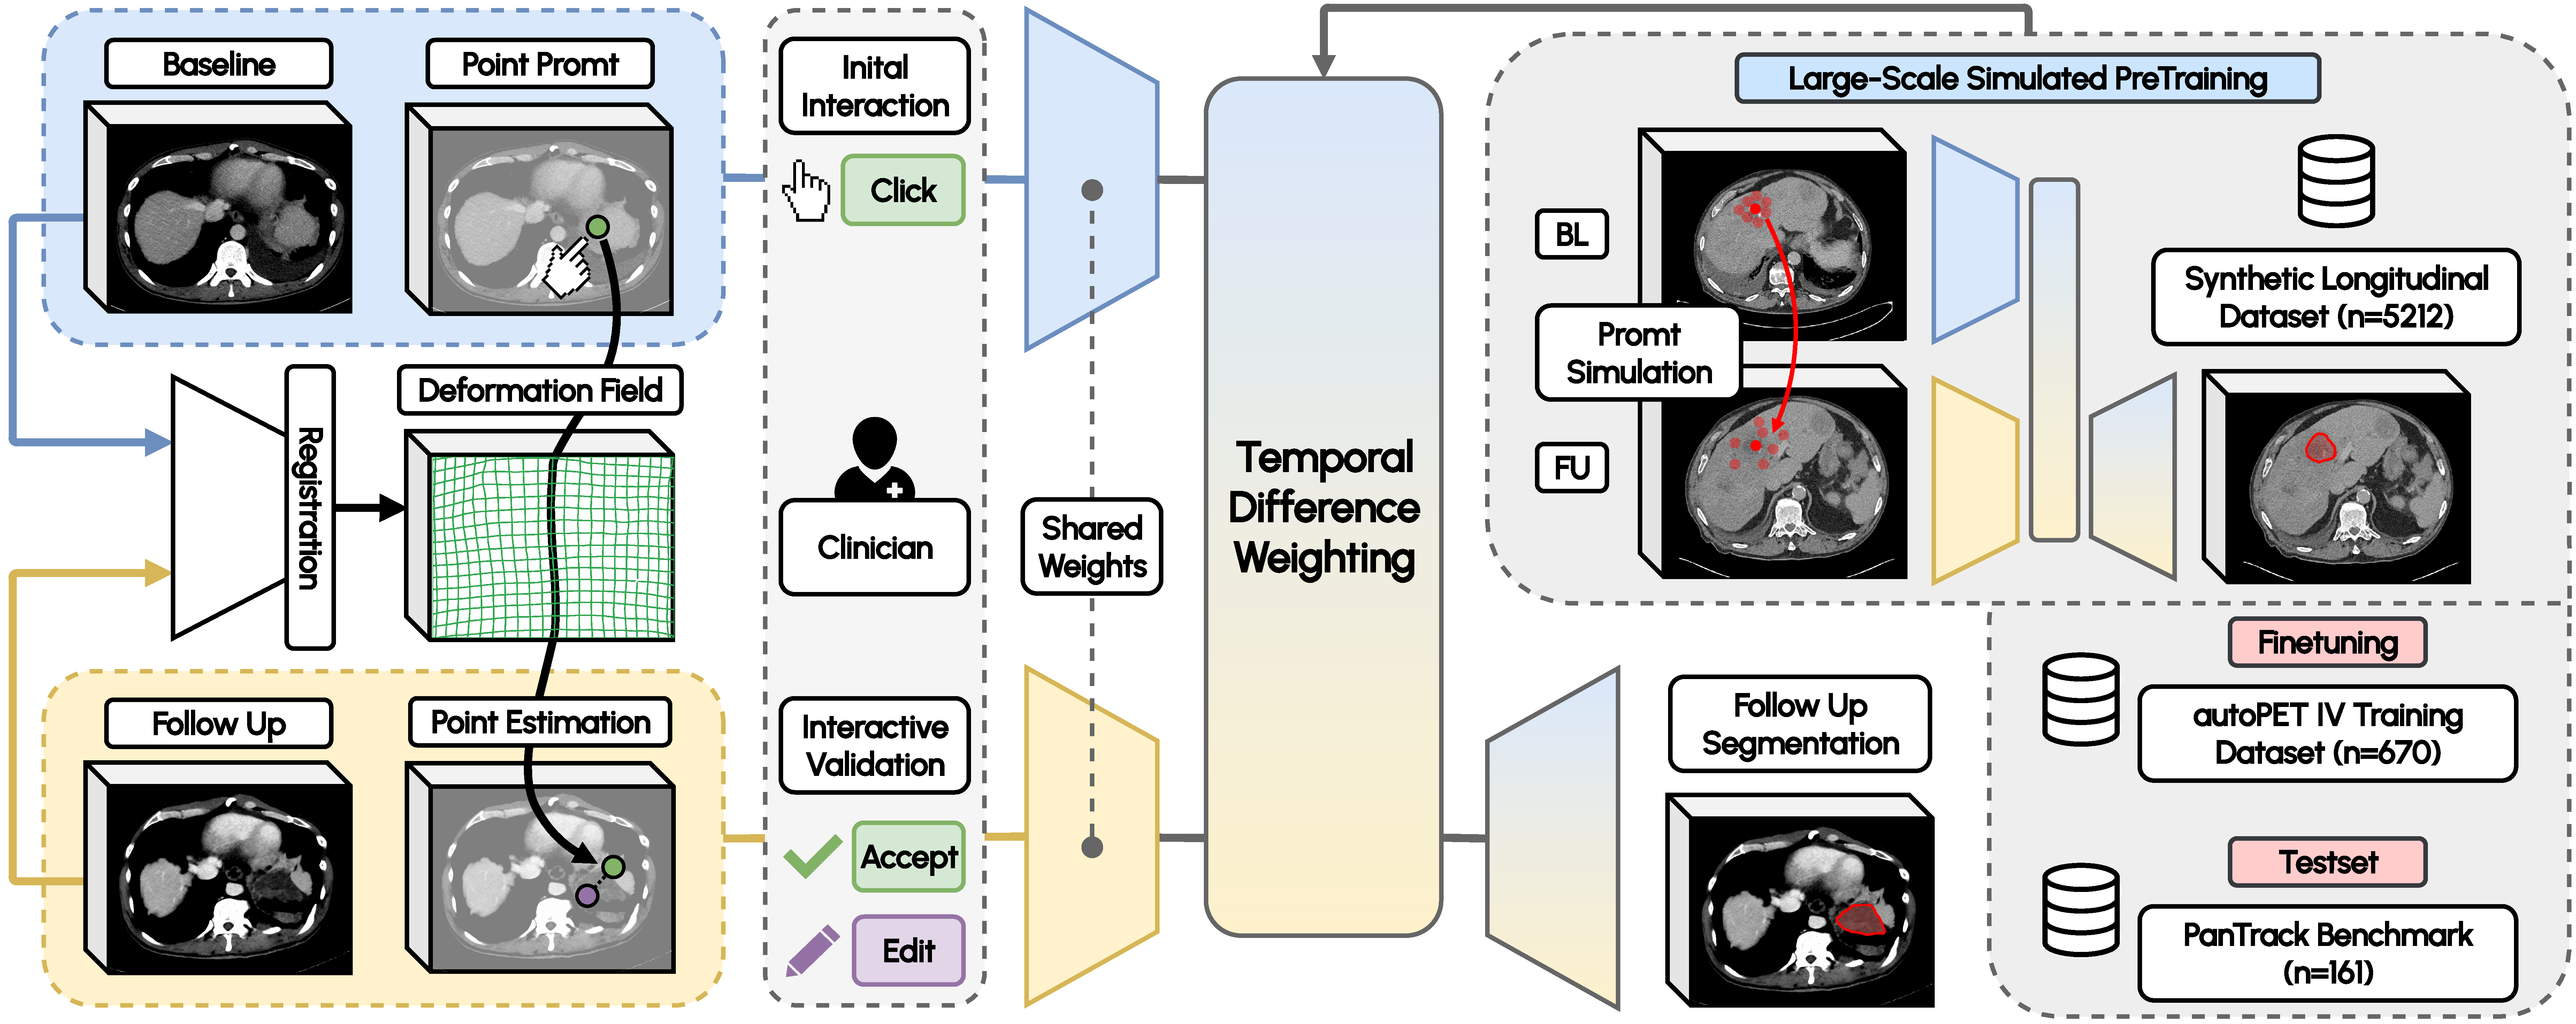
\includegraphics[width=1\textwidth]{figures/fig_1_overview.pdf}
\caption{\textbf{Overview of our framework.} The registration proposes a candidate follow-up prompt which the clinician verifies or corrects. A shared-weight encoder processes both (image, prompt) pairs and in latent space a Difference Weighting Block fuses their features by explicitly attending to temporal change before the decoder produces the longitudinally-informed follow-up segmentation. Prior, the model is pretrained on a large-scale synthetic longitudinal corpus with simulated prompts for both timepoints.}
\label{fig:overview}
\end{figure}

\subsection{Problem Formulation}

Given a baseline CT scan $I_0$ with a known lesion center $p_0$ and a follow-up CT scan $I_t$, our goal is to produce a volumetric segmentation of the corresponding lesion in $I_t$, conditioned on a clinician-verified follow-up point prompt $p_t$.

\subsection{Verified Tracking via Registration}

We decouple the longitudinal tracking workflow into two stages: (1)~a \textit{retrieval} step, handled jointly by a registration model and the clinician, and (2)~a \textit{delineation} step, performed by our segmentation network. For the retrieval step, we apply uniGradICON~\cite{uniGradICON}, a registration foundation model trained across diverse anatomical regions, to estimate a deformation field $\phi: I_0 \to I_t$, yielding a candidate follow-up prompt:
\begin{equation}
    \hat{p}_t = \phi(p_0).
\end{equation}
The clinician views $\hat{p}_t$ superimposed on $I_t$ and either accepts it or provides a corrected $p_t$. This verification step eliminates retrieval failures while preserving a high degree of clinical automation. For the autoPET IV dataset, the provided registration-propagated center points~\cite{kuestner2025longitudinalct} serve directly as $\hat{p}_t$.


\subsection{Segmentation Network Architecture}

Unlike decoupled pipelines that segment the follow-up in isolation, our model conditions delineation on both $(I_t, p_t)$ \emph{and} $(I_0, p_0)$, explicitly learning to use baseline appearance to resolve ambiguities that a single-timepoint model cannot. Our segmentation network must simultaneously handle two distinct integration challenges: incorporating a \textit{spatial point prompt} and leveraging \textit{baseline appearance}. These two signals empirically demand fusion at different levels of abstraction: spatial prompts are most effective at the image input level~\cite{nnInteractive,scribbleprompt}; longitudinal context requires latent-space integration with an explicit inductive bias towards temporal differences to prevent the network from ignoring the baseline branch altogether~\cite{longiseg,denner2020spatio}. We combine both in a Residual Encoder U-Net~\cite{nnunet_revisited} with the hybrid fusion design below.\\


\noindent\textbf{Early Prompt Fusion.}
After verified registration, we extract Volumes of Interest (VOIs) centered at $p_0$ and $p_t$ from $I_0$ and $I_t$, respectively. Following prior findings that prompt encoding is most effective at the input level~\cite{nnInteractive, scribbleprompt}, we concatenate image and prompt channel-wise:
\begin{equation}
    X_0 = [I_0,\; G(p_0)], \quad X_t = [I_t,\; G(p_t)],
\end{equation}
where $G(p)$ denotes a Gaussian heatmap with $\sigma=1$ centered at $p$, rescaled to unit value at the center. Crucially, $p_t$ does not need to lie precisely at the lesion center; residual registration error or clinical corrections are explicitly anticipated. Both pairs are then processed by a \textit{shared-weight} encoder, yielding multi-scale features $\{x_0^l\}$ and $\{x_t^l\}$ at each resolution level $l$.\\

\noindent\textbf{Latent Temporal Fusion via Difference Weighting.}
Naive channel-wise concatenation of multi-timepoint features risks the network primarily attending to a single timepoint, effectively collapsing to cross-sectional behavior~\cite{longiseg,denner2020spatio}. To impose an explicit longitudinal inductive bias, we apply a Difference Weighting Block (DWB)~\cite{longiseg} at all U-Net skip connections. For baseline and follow-up features ($x_0^l$, $x_t^l$), the DWB computes:
\begin{equation}
    {x'}_t^{\,l} = x_t^l \;\times\; \mathrm{InstNorm}\!\left(x_t^l - x_0^l\right) + x_t^l.
\end{equation}
The normalized feature difference acts as an attention map, gating $x_t^l$ to emphasize regions of longitudinal change. This lightweight operation runs at all resolutions without architectural overhead. The temporally-informed features $\{{x'}_t^l\}$ are passed to the decoder to generate the follow-up segmentation. To our knowledge, this is the first framework to combine early prompt fusion with latent temporal fusion, applying each mechanism precisely where it is most effective.\\


\noindent\noindent\textbf{Synthetic Longitudinal Pretraining.}
Real annotated multi-timepoint data is scarce, and without sufficient
training data even a longitudinal architecture can collapse
to cross-sectional behavior, ignoring the baseline scan entirely.
We address this by extending the synthetic corpus of~\cite{Rokuss_2025_CVPR}
to the promptable setting: 2{,}606 CT pairs with synthetic follow-ups
generated via anatomy-informed deformation fields~\cite{kovacs2023anatomy} simulating tumor
growth, shrinkage, and acquisition variability are paired with full
prompt simulation for both timepoints.\\


\noindent\textbf{Prompt Simulation.} To instill robustness against imprecise user interactions and registration errors, training prompts are generated via a 50/50 split: half are sampled from the ground-truth mask with probabilities weighted by $1/d^2$, where $d$ is the distance to the centroid, and half are derived from the registered follow-up point, which may even fall outside the lesion.

